\section{Impact of KID non-linearity}
\label{se:KID_NL}

\subsection{Total power}

In this paragraph we characterize KID non-linearity in total power. To do so, we simulate the observation of a point source by a KID, with a flux that we vary between \todo{1 and 2000\,Jy TBC} (fluxes are unrealistically large on purpose for illustration), to see how linear the measure remains. We assume that our instrument has a 11\,arcsec FWHM Gaussian beam like the polarized 1\,mm channel of \nikad. In the simulation, we use \methodu\ and  \methodd\ to recover the received power. We write the non linear detector response as :

\begin{equation}
m = m + \varepsilon_{det} m^2 +c_{0}.
\label{eq:model_kid_nl}
\end{equation}

\epsDET\ represents the non linearity of the KID. 
For all simulations we compute the non-linearity coefficient \epsDET\ from eq.~(\ref{eq:model_kid_nl}) by doing a linear fit of the input fluxes as a fonction of output fluxes.

Fig.~\ref{fig:planet_profiles} and Fig.~\ref{fig:flux_out_vs_in} show that under a bright source, non-linearity appears with the distortion of the input gaussian profile in the case of \methodu\ whereas \methodd\ remains linear on the same flux scale. The non-linearity coefficients that we find with \methodu\ and \methodd\ are respectively \epsDET =$-2.22 \times 10^{-5}$ and \epsDET =$8.69 \times 10^{-8}$. 



\begin{figure}
  \includegraphics[clip, angle=0, width=\columnwidth]{Figures/planet_profiles_2.eps}
  \caption{Comparison of an incoming flux that we vary between 1 and 2000 Jy TBC (in black), with flux reconstructed by \methodu\ and \methodd. Fluxes are unrealistically large on purpose for illustration. }
  \label{fig:planet_profiles}
\end{figure}


\begin{figure}
  \includegraphics[clip, angle=0, width=\columnwidth]{Figures/flux_out_vs_in.eps}
  \caption{Comparison of an incoming flux that we vary between 1 and 2000 Jy TBC (in black), with flux reconstructed by \methodu\ and \methodd. Fluxes are unrealistically large on purpose for illustration. }
  \label{fig:flux_out_vs_in}
\end{figure}


Simulations of a KID non-linearity in total power meets the requirements (see Sec.~\ref{cmb}) necessary to not biais measures of B modes. In CMB polarization experiments, the use of Half Wave Plate to modulate polarization are more and more considered. In the next section we will study the effect that can have this signal on the KID linearity.

\subsection{Polarization and Half Wave Plate}
\subsubsection{Half Wave Plate}

%\begin{itemize}
%\item les HWP deviennent a la mode
%\item les kids ont des constantes tres petites, donc on peut faire tourner vite
%  : avantages...
%\item ... mais signal parasite tres fort et donc besoin de le soustraire et de
%  voir si il n'induit pas de non linearite sur la mesure du signal
%\item simulations du \mathcal{H} (beta): bien expliquer que ce qui compte c'est la
%  subtraction of this template not the exact recovery of the input model
%\item which constraints do we set on the \mathcal{H} subtraction and potential
%  improvement if we could use hundreds of KIDS rather than just fit it kid by kid
%\item anticipate a bit on the achieved residual NL on the same planet as in the
%  previous section.
%\item simulate the sum of a template and pure weak signal and see the induced NL
%  on the signal
%\item comparison to NIKA(2)'s data... vs Simon's observatory perspectives
%\end{itemize}

%{\color{blue}
%Modulation of the polarization by a rotating Half Wave Plate (HWP) like in
%\nika\ and \nikad\ creates a background modulation equivalent to several tens to
%hundreds of Jy at frequencies close to the HWP rotation harmonics
%\citep{2017A&A...599A..34R}. After early tests by \todo{cite Hildebrand in the
%  80's or so ?}, this kind of modulating device has been left aside for
%\todo{20~TBC} years in the context of millimetric observations. With the
%improvement of technologies it progressively came back in the landscape, in
%particular with pioneering experiments like \emph{Maxipol}
%\citep{2007ApJ...665...42J} and \emph{EBEX} \citep{2010SPIE.7741E..1CR}. It is
%now more and more common and is considered as the leading option for future
%satellite designs such as \emph{LiteBIRD} \todo{add ref}. Such a background must
%be accounted for in the simulations.}

After early tests by \citep{1984ApJ...284L..51H}, modulation of the polarization by a rotating Half Wave Plate (HWP) has been left aside for \todo{20~TBC} years in the context of millimetric observations. With the improvement of technologies it progressively came back in the landscape, in particular with pioneering experiments like \emph{Maxipol} \citep{2007ApJ...665...42J}, \emph{SPIDER} \citep{2008SPIE.7010E..2PC}, \emph{EBEX} \citep{2010SPIE.7741E..1CR}, \emph{Polarbear} \citep{2012SPIE.8452E..1CK} \emph{BLAST-Pol} \citep{2014MNRAS.437.2772M}, \emph{ABS} \citep{2014RScI...85c9901K} and \emph{Advanced ACTPol} \citep{2016JLTP..184..772H}. It is now more and more common and is considered as the leading option for future satellite designs such as \emph{LiteBIRD} \citep{2014JLTP..176..733M} and next generation ground based experiments such as \emph{CMB-S4} \citep{2016arXiv161002743A}. The rotation of the HWP can be stepped (\emph{POLARBEAR} \citep{2014ApJ...794..171P}) or continuous  (\emph{EBEX}, \emph{ABS} and \nikad\  \citep{2015fers.confE..16R}). There exist different mechanism to rotate a HWP. For example, the HWP of \nikad\ is mounted inside a holder and coupled with a step motor, whereas \emph{EBEX} HWP is levitated with a superconducting magnetic bearing.
Using a HWP to modulate the polarization is a powerful tool to mitigate several instrumental systematics \citep{2009MNRAS.397..634B}. In fact, with a HWP :

\begin{itemize}
\item The polarized signal is modulated at 4 times the rotation frequency of the HWP and therefore is shifted at higher frequencies, isolating it from electronic noise and 1/f noise. This is valid if the rotation of the HWP is continous and fast ( HWP rotation frequency of \emph{EBEX} and \nika\ are respectively 1.235 Hz \citep{2018ApJS..239....7T} and 2.98 Hz \citep{2017A&A...599A..34R}.)

\item A single detector $k$ can measure a combination of the three Stokes parameters $I$, $Q$ and $U$ :

\begin{equation}
\label{eq:polar_measure}
m_{k}(t) = \frac{1}{2} [I + \rho [Q \cos (4 \omega t + 2 \alpha(t)) + U \sin (4 \omega t + 2 \alpha(t))]],
\end{equation}

with $\alpha$ the angle between the telescope reference frame and the local meridian on the sky and $\omega t$ is the position angle of the HWP.
This allows to do observations without having to use differencing polarization sensitive detectors and thus avoid systematic effects such as intensity to polarization leakage from mismatch of the detector beams \citep{2008PhRvD..77h3003S, 2015ApJ...814..110B}

\item We can achieve an optimal angular coverage as each pixel will be observed over a wide range of orientations. This allows to have a better angular redundancy in a single pixel to measure the Stokes parameters without having to rotate the full instrument.
\end{itemize}

On the downside, this kind of modulation can give rise to a systematic effect that is specific to instruments using a continuously rotating HWP : the Half Wave Plate Synchronuous Signal (HWPSS). In the next paragraph, we study non-linearity that are induced by this additional signal.

\subsubsection{Half Wave Plate Synchronous Signal}

\begin{figure}[h]
\center
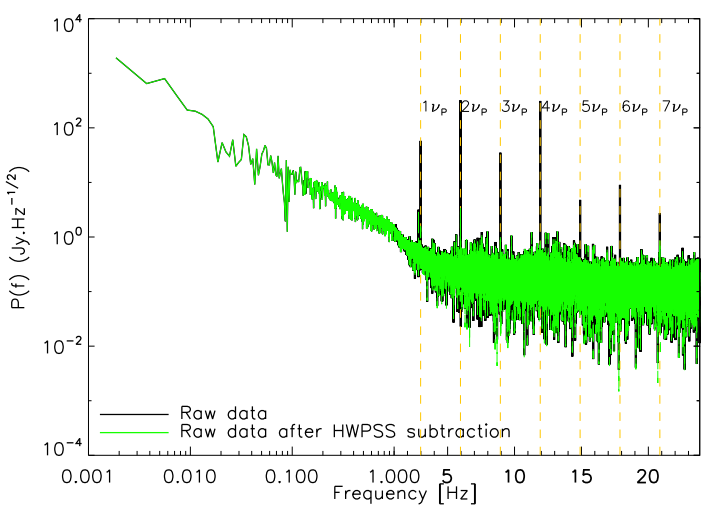
\includegraphics[clip, angle=0, width=\columnwidth]{Figures/hwp_power_spectrum.png}
\caption{Power spectrum of an observation of Orion OMC-1 for one KID. The parasitic signal is highly peaked at harmonics of the HWP rotation frequency. The observations were done with \nika . Black and green lines represent respectively the raw data and the raw data after subtraction of the HWP parasitic signal \citep{2017A&A...599A..34R}. }
\label{fig:hwp_power_spectrum}
\end{figure}

\begin{figure}[h]
\center
\includegraphics[clip, angle=0, width=\columnwidth]{Figures/hwpss_2pi.eps}
\caption{Representation of the parasitic signal as a function of angles of the HWP. The points are gathered around precise values of angles because the acquisition is synchrnous with the HWP rotation. Red dots correspond to the points reconstructed by the model of eq.~\ref{eq:hwp-template}. Blue curve corresponds to the model on one period.}
\label{fig:hwpss_2pi}
\end{figure}

Non-idealities of the HWP can create a background modulation equivalent to several tens of Jy at frequencies close to the HWP rotation harmonics \citep{2017A&A...599A..34R} (see Fig.~\ref{fig:hwp_power_spectrum} and Fig.~\ref{fig:hwpss_2pi}). This HWP synchronous signal (HWPSS) was observed by \emph{MAXIPol} \citep{2007ApJ...665...42J}, \emph{EBEX} \citep{2010SPIE.7741E..1CR}, \emph{POLARBEAR} \citep{2017JCAP...05..008T} and \nika\ \citep{2017A&A...599A..34R}, although they have different HWP and HWP rotation mechanism. This signal must be subtracted from observations or it will dominate polarization. To do that, we can model it by a sum of $n$ harmonics of the HWP rotation frequency $\nu_{p}$ with amplitudes $A_{n}$ and $B_{n}$ that are linearly drifting :

\begin{equation}
\mathcal{H}(t) = \sum_{n=1} A_{n} \cos n\omega t + B_{n} \sin n \omega t , 
\label{eq:hwp-template}
\end{equation}

where : 
\begin{eqnarray}
A_{n}  &=& A_{n}^{0} + \varepsilon_{A_{n}}t,\\
B_{n}  &=& B_{n}^{0} + \varepsilon_{B_{n}}t, 
\end{eqnarray}

with $\omega = 2 \pi \nu_{p}(t)$.
This effect can then be corrected by subtracting observations by the model presented in eq.~\ref{eq:hwp-template}. 

A large amplitude of $\mathcal{H}(t)$ could bias the measurement and the photometry by causing non-linearity in the detector response. This non-linear response can then be the source of coupling between intensity and polarization signals. Systematic effects arising from detector non-linearity have been studied in \emph{Simon's Observatory} \citep{2018SPIE10708E..48S}, \emph{POLARBEAR} \citep{2017JCAP...05..008T} and \emph{EBEX} \citep{2017arXiv171101314D}. In the latter, it was shown that the dominant source of intensity to polarization leakage is due to detector non-linearity caused by a large HWPSS \citep{2017arXiv171101314D}.

In \nikad\ this additionnal noise is two to three order of magnitude above the noise level, making it one of the strongest noise contributor in polarization observations, such a bakground must be accounted for in the simulations. In the next paragraph, we study the non-linearity of a KID caused by a large HWPSS. 

\subsubsection{Simulations}

In our simulation, we test the impact of this parasitic signal on the observations and if the residuals left by the subtraction of $\mathcal{H}$ can create non-linearity. We keep the instrumental parameters of Sect.~\ref{se:kids} and we simulate the observation of a point source, with a flux that varies between 1 and 500 Jy. To account for the parasitic signal $\mathcal{H}$, we build a template following eq.~\ref{eq:hwp-template}, with a maximum amplitude of 70 Jy as seen in \nikad , that we add to the observation. To subtract this additional signal, we fit the template $\mathcal{H}$ by using the method described in \citep{2017A&A...599A..34R}, and then subtract it to our observation. We use the same method as in Sec.~\ref{se:kids} to derive the non-linearity coefficient \epsDET . Fig.~\ref{fig:histos_epsilon_rf} and Fig.~\ref{fig:histos_epsilon_cf} show the distribution of non-linearity coefficients for different method of signal reconstruction (\methodu\ and \methodd). For one realization we vary the amplitudes $A_{n}$ and $B_{n}$ of $\mathcal{H}$.

\begin{figure}
	\includegraphics[clip, angle=0, width=\columnwidth]{Figures/histos_epsilon_rf.eps}
	\caption{Histogram of non-linearity coefficients derived with \methodu\ and scanning speed equal to 3 and 5 points per beam.}
	\label{fig:histos_epsilon_rf}
\end{figure}

\begin{figure}
	\includegraphics[clip, angle=0, width=\columnwidth]{Figures/histos_epsilon_cf.eps}
	\caption{Histogram of non-linearity coefficients derived with \methodd\ and scanning speed equal to 3 and 5 points per beam.}
	\label{fig:histos_epsilon_cf}
\end{figure}

The mean value of non-linearity coefficient derived with \methodu\ and \methodd\ are respectively \epsDET = $-2.2 \times 10^{-5}$ and \epsDET =  $-4.7 \times 10^{-7}$, this show that as precedently, \methodd\ remains more linear than \methodu\ on the same flux scale. We manage to correctly subtract the HWPSS template so that it doesn't create additional non-linearities, in fact, with both methods, the non-linearity coefficients are of the same order of magnitude with or without the additional HWPSS template. The non-linearity coefficients derived from the simulations are lower than the non-linearity coefficient required in Sect.~\ref{sec:cmb} to detect B modes without being biaised by non-linearity arising from the detector and the HWPSS. 
In these simulations, we have shown that non-linearity appears when the detector is under a bright source, leading to a poor reconstruction of the signal. In the next section, study realistic simulations by using a scanning strategy typical of a satellite to scan the Galaxy which is more complex than a planet and to ensure that its signal can be reconstructed with \methodu\ and \methodd .
